\section{\cyclus}
\label{sec:cyclus}
% fix that, too informal and introduces archetypes without context.
\cyclus is an agent-based \gls{nfc} simulator that is versatile, open source, and modular. The software achieves this versatility through a series of generic archetypes that are primarily transaction based. Over the years, the user community and developers have created a litany of nuclear specific archetypes for everything from proliferation assessment to fuel burnup. Many standard fuel cycle facilities have been implemented in the \cycamore repository on GitHub, which holds technology-agnostic archetypes for material sources, material sinks, enrichment services, separations capabilities, and a generic reactor.

% discuss recipes
As \cyclus is a transactions code and not necessarily a physics code,
the reactors incorporate reactor physics through pre-defined "recipes,"
where the user specifies the isotopic concentration of the fresh and
used fuel.

Users approximate the burnup of each fuel element with the
same input recipe as the same; however, in this work we incorporate a
cascading enrichment from \gls{leu+} to \gls{haleu}.
% find a citation or source that companies are actually going to do that
% (best case scenario is find it for each reactor you do it for)

% discuss EVER and CLOVER?
Novel in this work is our use of a low fidelity archetype based on the
\cycamore reactor %\cite{the summer poster}. \gls{ever}

\gls{ever} allows the user to specify multiple recipes for the fuel and
change between them at specific times.


% discuss DRE
As we have discussed, \cyclus's primary function is to keep track of
material transactions between agents. This is accomplished through the
\gls{dre}, which functions like a market where each agent brings a bid
for what and how much material they need and suppliers are matched with
buyers % cite something here.


\subsection{Archetypes and Time Management}
\label{sec:archetypes_and_time_management}

Throughout the \cyclus ecosystem, archetypes interact with the \gls{dre} and each other in a fixed, user defined, time step, forcing the entire simulation to operate on the smallest universal time step. For example, if a fabrication facility can produce material every 2 months but the enrichment facility can only provide material every 3 months, then we would need to use a 1 month time step to capture both. When the time step is smaller than the minimum for a given facility, that facility still participates in the \gls{dre} with a 0 bid. These zero bids, across hundreds of facilities, add complexity and inefficiencies to solving the transaction problem at each time step.

Examining the \cyclus ecosystem, we identified an archetype called $Pattern_Sink$ wherein the user can alter the frequency that the material sink, often called the repository, can accept material. We have created an example of this archetype in action with a simple A-B-C scenario, shown in Figure \ref{fig:a-b-c}. In this scenario, material is received from a source (A) to a reactor (B) with a final (C) sink that can only accept material at a certain frequency.

\begin{figure}
    \centering
    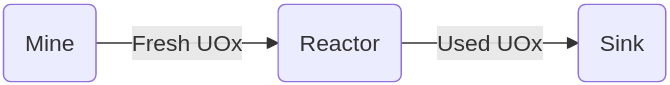
\includegraphics[scale=0.4]{images/cyclus/a-b-c.png}
    \caption{Simple A-B-C Scenario}
    \label{fig:a-b-c}
\end{figure}

If we track the material being received by the sink it becomes clear that this frequency simply alters how frequently the archetype updates its internal understanding of time. As a consequence, it appears in Figure \ref{fig:pattern_freq_50} as though multiple groups of material are received in one time step despite this archetype not having an idea of individual shipments. The way this archetype accomplishes the artificial restriction on accepting material is by simply not updating the time step that the archetype is at until the next universal time step is met. Regardless of function, this is the only example of flexibility of timestep we found in the ecosystem.

\begin{figure}
    \centering
    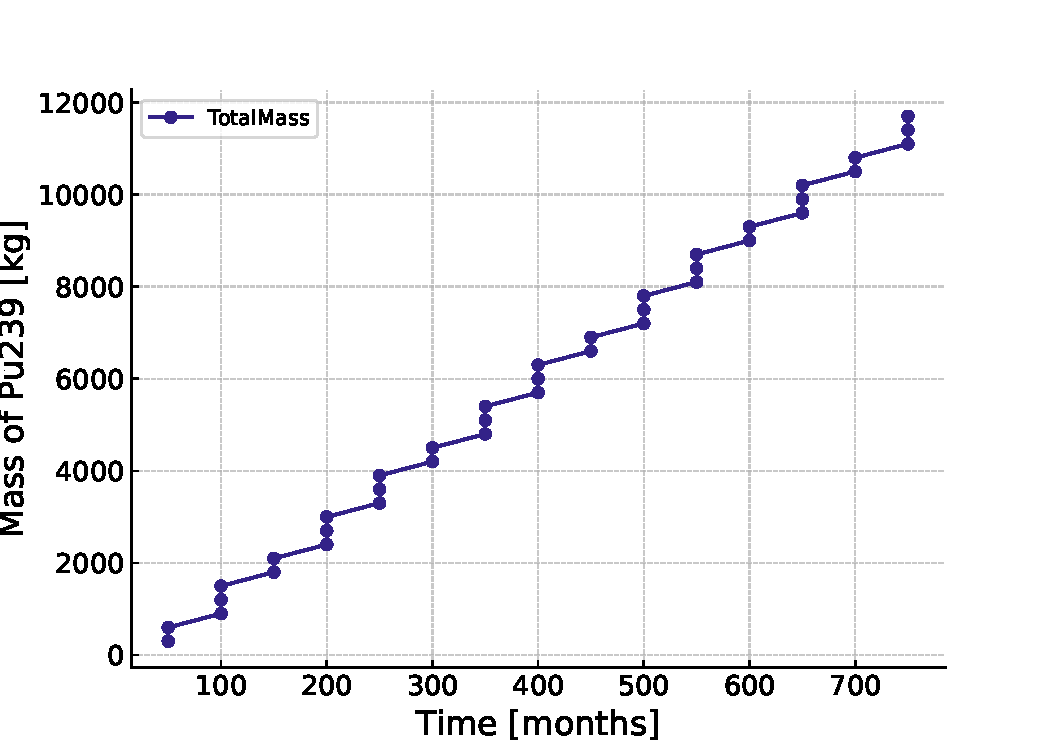
\includegraphics[scale=0.4]{images/cyclus/pattern_sink_fuel_transactions.pdf}
    \caption{Production of $^{239}$Pu with a frequency of 50 months}
    \label{fig:pattern_freq_50}
\end{figure}

In this work we implement a fundamental toolkit capability that any archetype in the Cyclus ecosystem can take advantage of with one implementation.
